\chapter{Basisbegrippen}
\label{sec:Basisbegrippen}

%%%%%%%%%%%%%%%%%%%%%%%%%%%%%%%%%%%%%%%%%%%%%%%%%%%%%%%%%%%%%%%%%%%%%%%%%%%%%%%%%%%%%%%
	\section{Inleiding}
	\label{sec:Basisbegrippen Inleiding}
Overal rondom ons vinden we vloeistoffen en gassen, fluïda. In deze cursus zullen we de bewegingen die deze fluïda ondergaan en de krachten die ze op de omgeving uitoefenen bestuderen. Vaak zullen ingenieurs deze krachten en bewegingen kanaliseren en uitbuiten om een bepaald doel te realiseren, bijvoorbeeld arbeid opwekken of een kracht uitoefenen of simpelweg de verplaatsing van massa van één locatie naar een andere. Om systemen die dit doen te ontwerpen is het nodig het gedrag van de fluïda in bepaalde omstandigheden goed te kunnen voorspellen.

Een bepaalde hoeveelheid fluïdum zal steeds bestaan uit een zeer groot aantal moleculen. De hoeveelheid moleculen binnen 1\unit{m^3} water bij atmosfeer druk en 20\degC\ is ongeveer $10\times10^{30}$. Een theorie die het gedrag van al deze moleculen zou voorspellen, bijvoorbeeld op basis van deeltjesmechanica, zou zeer complex zijn en weinig praktisch nut hebben aangezien de rekencapaciteit van huidige supercomputers verre van voldoende zou zijn om zulke systemen op te lossen.

We moeten dus methodes bedenken om het globale gedrag van zulke systemen te beschrijven.

In dit hoofdstuk worden enkele principes uitgewerkt die het mogelijk maken om fluïda te bestuderen.
	
%%%%%%%%%%%%%%%%%%%%%%%%%%%%%%%%%%%%%%%%%%%%%%%%%%%%%%%%%%%%%%%%%%%%%%%%%%%%%%%%%%%%%%%
	\subsection{Beschrijving van een continuüm}
	\label{sec:Beschrijving van een continuum}	
We zullen binnen de fluïdomechanica een fluïdum niet bestuderen als een verzameling van moleculen maar als een continuüm. Deze benadering is analoog aan degene gebruikt binnen de vaste stof mechanica. We smeren als het ware de moleculen binnen het fluïdum uit over de volledige ruimte die het fluïdum inneemt (en niet enkel de ruimte die bezet wordt door de afzonderlijke moleculen). Dit brengt met zich mee dat alle afgeleide principes enkel geldig zijn indien we een volume beschouwen waarin voldoende moleculen aanwezig zijn zodat de gemiddelde eigenschappen van de aanwezige moleculen representatief zijn.

Beschouw als voorbeeld een bepaald volume uit een fluïdum. Aangezien de moleculen in een fluïdum een grote bewegingsvrijheid hebben zullen er steeds moleculen het volume in en uit bewegen. Wanneer het beschouwde volume echter groot genoeg is zullen er steeds ongeveer evenveel moleculen binnen het beschouwde volume zijn (de beweging van de moleculen is willekeurig dus zullen er evenveel moleculen instromen als uitstromen). De massa van het fluïdum binnen het volume is dus ook constant. Wanneer het volume echter zo klein gekozen wordt dat er slechts enkele moleculen zich binnen het volume bevinden heeft de verplaatsing van één enkele molecule een veel groter effect op de variatie van massa binnen het volume en kan de continuümaanname niet meer gerechtvaardigd worden.

Een belangrijke eigenschap voor het beschrijven van een continuüm is de \emph{massadichtheid} of \emph{dichtheid}. Deze wordt gedefinieerd als de massa binnen een bepaald volume gedeeld door het ingenomen volume wanneer dit volume infinitesimaal klein wordt. 
\begin{equation}
	\rho = \lim_{\delta V \to 0} \frac{\delta m}{\delta V}
	\label{eqn:dichtheid}
\end{equation}
Onder de continuümaannames zal de dichtheid onafhankelijk zijn van de grootte van het infinitesimaal volume en heeft de bovenstaande limiet een constante waarde. De SI eenheid van dichtheid is \unit{kg/m^3}.

In de mechanica zijn we steeds geïnteresseerd in de beweging en vervorming van systemen onder invloed van krachten. In de continuümveronderstelling kunnen we deze krachten onderverdelen in \emph{volumekrachten} en \emph{oppervlaktekrachten}. De meest voor de hand liggende volumekracht is de zwaartekracht. Deze zal overal in het continuüm aangrijpen en is gelijk aan het product van de massadichtheid en de valversnelling. De totale kracht die een volumekracht uitgeoefend op een systeem kunnen we berekenen door de volume-integraal van de volumekracht over het volledige volume te nemen (vandaar de naam). Zo wordt de totale zwaartekracht uitgeoefend op een systeem:
\begin{equation}
	\vt{F_{g,totaal}} = \int_V \rho \vt{g} \diff V = m \vt{g}
	\label{eqn:volumekracht}
\end{equation}
In tegenstelling tot volume krachten zullen oppervlaktekrachten enkel aan de rand van een volume inwerken. Deze kunnen beschreven worden door de spanning op een oppervlak. De spanning noteren we met het symbool $\sigma$ of $\tau$ en heeft een eenheid  \unit{N/m^2}. De totale kracht die een spanning op een oppervlak uitoefent wordt berekend als: 
\begin{equation}
	\vt{F_{\sigma,totaal}} = \int_A \vt{\sigma} \diff A
	\label{eqn:oppervlaktekracht}
\end{equation}
De spanning op een oppervlak kan steeds beschreven worden door een component loodrecht op het oppervlak, de \emph{normaalspanning} $\sigma$ en een component tangentieel aan het oppervlak, de \emph{schuifspanning} $\tau$ (Figuur \ref{fig:spanning}).
\begin{figure}[htb]
	\centering
	\includesvg{fig/basisbegrippen/Spanning}
	\caption{Spanning aan het oppervlak van een continuüm}
	\label{fig:spanning}
\end{figure}

%%%%%%%%%%%%%%%%%%%%%%%%%%%%%%%%%%%%%%%%%%%%%%%%%%%%%%%%%%%%%%%%%%%%%%%%%%%%%%%%%%%%%%%
	\section{Beschrijving van een fluïdum}
	\label{sec:Beschrijving van een fluidum}
Beschouw twee starre evenwijdige platen op een bepaalde afstand van elkaar met een bepaald fluïdum ertussen (Figuur \ref{fig:Evenwijdige platen}). De onderste plaat staat vast opgesteld, terwijl de bovenste plaat kan bewegen zoals aangegeven op de figuur. Indien we een kracht $F$ uitoefenen op de bovenste plaat zal deze in dezelfde richting gaan bewegen. De uiteindelijke snelheid waarmee de plaat beweegt zal afhankelijk zijn van de uitgeoefende kracht.
\begin{figure}[htb]
	\centering
	\includesvg{fig/basisbegrippen/Viscositeit_platen}
	\caption{Evenwijdige platen met een vloeistof }
	\label{fig:Evenwijdige platen}
\end{figure}
Wanneer we de kracht uitoefenen zoals aangegeven introduceren we een spanning in de vloeistof met grootte $\tau$:
\begin{equation}
	\tau = \frac{F}{A}
\end{equation}
Met $A$ de oppervlakte van de vloeistof in contact met één van de platen. Aangezien deze ervoor zal zorgen dat de twee platen ten opzichte van elkaar gaan schuiven wordt hierdoor de naamgeving schuifspanning ook duidelijk. Indien we een schuifspanning op een vaste stof zouden uitoefenen via de twee platen, dan zouden deze over een bepaalde afstand $\delta$ verschuiven en dan tot stilstand komen. Bij een fluïdum zal de beweging echter niet stoppen. Hieruit volgt ook de definitie van een fluïdum:

\begin{quotation}
	Een fluïdum is een stof die onder invloed van een eindige kracht een oneindige vervorming aanneemt.
\end{quotation}

In de vaste stof mechanica wordt de vervorming tot de spanning gerelateerd door de elasticiteitsmodulus of de glijdingsmodulus. Aangezien er in de fluïdomechanica sprake is van oneindige vervormingen is een zelfde aanpak niet mogelijk. Een andere aanpak is de schuifspanning te relateren aan de vervormingssnelheid. Als in het beschouwde voorbeeld de bovenste plaat een snelheid $v_0$ heeft dan zal een deel van de vloeistof dat op tijdstip $t$ een rechthoekige vorm had er op een tijdstip $t+\Delta t$ eruitzien als een parallellogram (Figuur \ref{fig:Vervormingssnelheid}). We kunnen we de vervormingssnelheid uitdrukken als de verandering van de hoek $\alpha$.
\begin{figure}[htb]
	\centering
	\includesvg{fig/basisbegrippen/Viscositeit_vervormingssnelheid}
	\caption{Vervormingssnelheid}
	\label{fig:Vervormingssnelheid}
\end{figure}
Uit experimenten blijkt dat in de buurt van een wand elk fluïdum de snelheid van de wand aanneemt. De snelheid van de vloeistof aan de bovenwand is dus ook $v_0$. De vervormingssnelheid wordt dan:
\begin{equation}
	\text{vervormingssnelheid} = \lim_{\Delta t \to 0} \frac{\alpha}{\Delta t} \simeq \lim_{\Delta t \to 0} \frac{\delta}{h \Delta t} = \frac{v_0}{h}
\end{equation}
Wanneer het snelheidsprofiel niet lineair is kunnen we deze uitdrukking veralgemenen tot:
\begin{equation}
	\text{vervormingssnelheid} = \frac{\diff v}{\diff y}
\end{equation}
De eenvoudigste relatie tussen vervormingssnelheid en schuifspanning is een lineaire relatie. Het verband wordt dan:
\begin{equation}
	\tau = \mu \frac{\diff v}{\diff y}
	\label{eqn:schuifspanning newtoniaans}
\end{equation}
De evenredigheidsfactor $\mu$ wordt de \emph{dynamische viscositeit} of gewoon \emph{viscositeit} genoemd met als eenheid \unit{Pa\ s}. Vloeistoffen die aan (\ref{eqn:schuifspanning newtoniaans}) voldoen worden \emph{Newtoniaanse} vloeistoffen genoemd. Vele praktische en ingenieursvloeistoffen als water, lucht, smeerolie,... voldoen zeer goed aan deze relatie.

Vaak wordt de viscositeit voorgesteld als een \emph{kinematische viscositeit} $\nu$. Deze wordt bekomen door de dynamische viscositeit te delen door de dichtheid van het fluïdum:
\begin{equation}
	\nu = \frac{\mu}{\rho}
\end{equation}
De eenheid van de kinematische viscositeit is \unit{m^2/s}.

De viscositeit van een vloeistof is vaak sterk afhankelijk van de temperatuur. Wanneer we Figuur \ref{fig:dynamische viscositeit temperatuur} bestuderen valt op dat bij vloeistoffen de viscositeit daalt bij stijgende temperatuur, terwijl bij gassen de viscositeit stijgt bij stijgende temperatuur. Dit kunnen we verklaren door op te merken dat bij vloeistoffen de verschillende moleculen dicht bij elkaar gelegen zijn. De viscositeit wordt dus hoofdzakelijk veroorzaakt door intermoleculaire krachten of cohesie. Bij hogere temperaturen nemen deze cohesiekrachten en dus ook de viscositeit af. Bij gassen is de afstand tussen de moleculen groter en de moleculen bezitten elk een willekeurige snelheid. De viscositeit wordt dus veroorzaakt door impulsoverdracht door de moleculen. Aangezien bij stijgende temperatuur de moleculaire activiteit toeneemt zal ook de viscositeit toenemen.
\begin{figure}[htb]
	\centering
	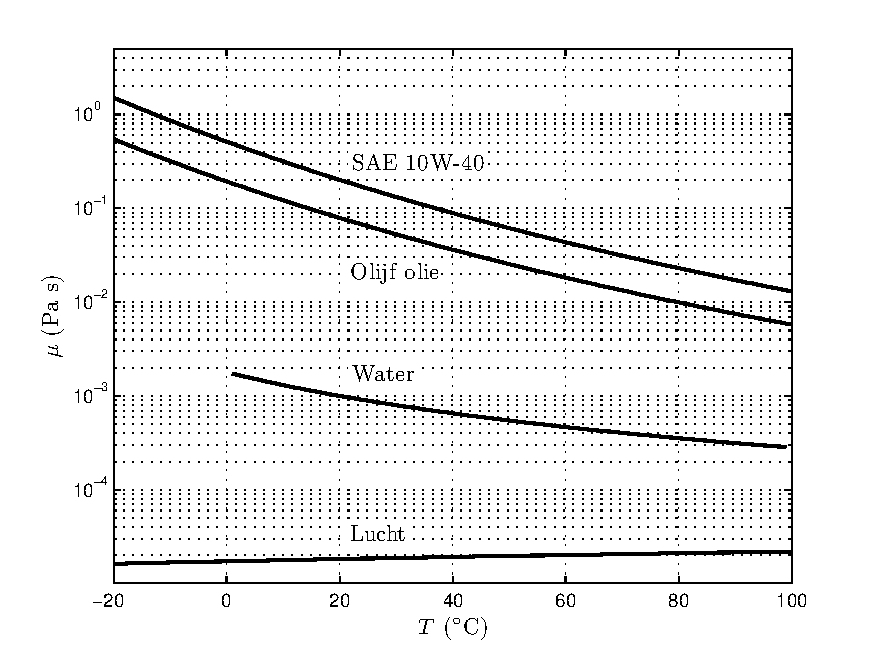
\includegraphics{fig/basisbegrippen/Dynamische_viscositeit_temperatuur.pdf}
	\caption{Viscositeit van verschillende fluïda met temperatuur}
	\label{fig:dynamische viscositeit temperatuur}
\end{figure}

In de literatuur zijn twee vaak gebruikte correlaties terug te vinden. Voor gassen geeft de \emph{Sutherland} vergelijking de relatie tussen dynamische viscositeit en absolute temperatuur:
\begin{equation}
	\mu = \frac{C T^{3/2}}{T+S}
\end{equation}
Met behulp van deze vergelijking kan de viscositeit bij eender welke temperatuur bepaald worden mits de kennis van viscositeit bij 2 temperaturen. Voor vloeistoffen wordt vaak gebruik gemaakt van de \emph{Andrade} correlatie:
\begin{equation}
	\mu = D e^{B/T}
\end{equation}
Ook hier zijn twee gekende punten noodzakelijk om de coëfficiënten in de vergelijking te bepalen. Een meer uitgebreide discussie over viscositeit en andere eigenschappen van fluïda is te vinden in \cite{Poling2001}.

%%%%%%%%%%%%%%%%%%%%%%%%%%%%%%%%%%%%%%%%%%%%%%%%%%%%%%%%%%%%%%%%%%%%%%%%%%%%%%%%%%%%%%%
	\section{Beschrijving van een stroming}
	\label{sec:Beschrijving van een stroming}
Wanneer een vloeistof stroomt wil dit zeggen dat er vloeistofdeeltjes zich verplaatsen van één plaats naar een andere. Deze beweging van deeltjes kunnen we beschrijven door de positie $\vt{r}$ van elk deeltje te volgen in de tijd. Indien we de positie van een deeltje op elk tijdstip kennen kunnen we ook de snelheid $\vt{v}$ van het deeltje bepalen en kunnen we de stroming karakteriseren. We kunnen dus elk deeltje een label $j$ geven en de snelheid en positie van elk deeltje beschrijven als:
\begin{eqnarray}
	\vt{r} = \vt{r}_j(t) \\
	\vt{v} = \vt{v}_j(t)
\end{eqnarray}
Deze benadering wordt de Langrange benadering genoemd en is bekend uit de deeltjesmechanica. Voor het behandelen van een continuüm is deze benadering echter niet erg praktisch. De hoeveelheid deeltjes die gevolgd zou moeten worden zou snel hoog oplopen.

Een andere benadering wordt de Euler benadering genoemd. Hier wordt de snelheid van de stroming beschreven als een vectorveld. Op elk tijdstip wordt op elke positie de snelheid bepaald onafhankelijk van welk deeltje er zich op dat tijdstip bevindt. Voor een tweedimensionale stroming wordt dit:
\begin{eqnarray}
	\vt{v} = \vt{v}(t,x,y)
\end{eqnarray}
Vaak zal het snelheidsveld onafhankelijk zijn van de tijd. Het snelheidsveld ziet er met andere woorden steeds hetzelfde uit. voor een tweedimensionale stroming wordt dit: 
\begin{eqnarray}
	\vt{v} = \vt{v}(x,y)
\end{eqnarray}
We noemen dit een stationaire stroming. Veel stromingen in de ingenieurstoepassingen kunnen als stationair beschouwd worden. De stroming van water door een leiding bijvoorbeeld zal op een inloop en uitloop fenomeen na tijdsonafhankelijk zijn. Ook de stroming door systemen als turbines en compressoren, met inwendig bewegende onderdelen, kunnen als stationair beschouw worden aangezien aan de inlaat en uitlaat de stroming weinig invloed zal ondervinden van het voorbijkomen van roterende onderdelen. Zolang we enkel in de ingaande en uitgaande stroming geïnteresseerd zijn is dit geldig. Wanneer we de details van de stroming in een turbine stator en rotor willen bestuderen zullen we deze als niet stationair moeten beschouwen.

Ook systemen die op het eerste zicht geen stationaire stroming ondervinden kunnen vaak door een slimme transformatie als stationair beschouwd worden. Nemen we als voorbeeld een vliegtuig. Aangezien het vliegtuig zich door de stilstaande lucht verplaatst zal op een gegeven moment de lucht plaats moeten maken voor het vliegtuig en voldoende tijd later terug in rust zijn. De stroming is dus duidelijk niet stationair. Indien we echter de stroming relatief ten opzichte van het vliegtuig bekijken dan zal het snelheidsveld rond het vliegtuig wel stationair zijn (Figuur \ref{fig:stationaire stroming vliegtuig}). 
\begin{figure}[htb]
	\centering
	\includesvg{fig/basisbegrippen/Stationaire_stroming_vliegtuig}
	\caption{Door een goede keuze van assenstelsel kan een stroming als stationair behandeld worden}
	\label{fig:stationaire stroming vliegtuig}
\end{figure}

Indien ze gekend zijn kunnen de snelheidsvectoren op elk moment grafisch weergegeven worden. Indien we een set lijnen tekenen die op elk punt raken aan de snelheidsvectoren kunnen we ook op deze manier de stroming grafisch weergeven. Deze lijnen worden \emph{stroomlijnen} genoemd (E: Streamlines). Als voorbeeld is in Figuur \ref{fig:snelheidsveld} een snelheidsveld gegeven voor een niet viskeuze stroming in een rechte hoek. De snelheidsvectoren worden als pijlen weergegeven op enkele discrete posities. De stroomlijnen zijn weergegeven als streeplijnen.
\begin{figure}[htb]
	\centering
	\includesvg{fig/basisbegrippen/Snelheidsveld}
	\caption{Weergave van het snelheidsveld van een niet-viskeuze stroming in een rechte hoek}
	\label{fig:snelheidsveld}
\end{figure}
Indien we een experimentele stroming willen visualiseren is het opmeten van de snelheidsveld niet eenvoudig. Een eenvoudige manier om een stroming te visualiseren is op bepaalde posities continu kleurstof te injecteren in de stroming. De lijnen die door de kleurstof gevormd worden kunnen weergegeven worden en worden \emph{stroombanen} genoemd (E: Streaklines).
Een andere manier is om op een bepaald tijdstip op bepaalde posities een kleurstof te injecteren in de stroming en het pad van de kleurstof te volgen. We volgen dan als het ware enkele vloeistofdeeltjes als in de Lagrange benadering. De gevormde lijnen worden \emph{padlijnen} genoemd (E: Pathlines).
Bij stationaire stromingen vallen de stroomlijnen, stroombanen en padlijnen samen.

		\subsection{Samendrukbaarheid van stromingen}
Elke stof zal wanneer er een druk op wordt uitgeoefend in zekere mate van volume veranderen. Bij vloeistoffen is deze verandering zeer klein of zelfs nauwelijks meetbaar zo zal water bij 20\degC\ en 200bar een dichtheid hebben die minder dan 1\% verschilt dan die van water bij 1bar. Gassen zijn daarentegen meestal goed samendrukbaar zo zal de dichtheid van lucht ongeveer verdubbelen ten bij een druk van 2bar ten opzicht van bij 1bar en gelijke temperatuur.

Ook al zijn vloeistoffen nauwelijks samendrukbaar, toch kunnen er zich drukgolven (zoals geluidsgolven) in voortplanten. De voortplantingssnelheid van een drukgolf in een bepaald medium wordt de \emph{geluidssnelheid} genoemd (E: speed of sound) en is afhankelijk van de toestand van de stof. In lucht bij 20\degC\ en atmosfeerdruk is de snelheid van het geluid ongeveer 340m/s. In water bij 20\degC\ en atmosfeerdruk  is dit ongeveer 1480m/s.

We zullen nu stromingen karakteriseren op basis van de dichtheidsveranderingen van het fluïdum. Wanneer de veranderingen zeer klein zijn spreken we van niet-samendrukbare stroming. Bij meetbare dichtheidsveranderingen kunnen we over samendrukbare stroming spreken. Merk meteen op dat volledig niet samendrukbare stroming een idealisering van de werkelijkheid is. Vaak zullen de dichtheidsveranderingen zo klein zijn dat ze geen invloed hebben op de rest van de stromingseigenschappen, de vereenvoudiging is dan verantwoord.

Algemeen kunnen stromingen als niet samendrukbaar beschouwd worden als de voorkomende snelheden veel kleiner zijn dan de snelheid van het geluid. Als praktische richtlijn wordt genomen dat indien de vrije stroomsnelheid kleiner is dan 20\% van de geluidssnelheid de effecten van samendrukbaarheid verwaarloosbaar zijn \cite{Durst2008}.

Uit deze beschouwingen kunnen we besluiten dat stromingen van water bijna steeds als niet-samendrukbaar behandeld kunnen worden. Zelfs stromingen in lucht bij snelheden tot 70m/s, zoals stromingen in ventilatiekanalen of zelfs rond auto's kunnen als niet samendrukbaar beschouwd worden. Er zijn echter uitzonderingen waarbij de samendrukbaarheid van vloeistoffen tot uiting komt. Zo zal wanneer in een waterleiding een afsluitkraan zeer snel wordt gesloten er een drukgolf ontstaan die de leiding of systemen ermee verbonden kunnen beschadigen \cite{Ghidaoui2005}. Dit fenomeen wordt \emph{waterslag} (E: water hammer) genoemd.

In deze cursus zullen we enkel stromingen behandelen die als niet samendrukbaar beschouwd kunnen worden.

		\subsection{Viskeuze stromingen}
Hoewel alle fluïda viskeus zijn kunnen sommige stromingen als niet-viskeus beschouwd worden. Merk namelijk op dat er enkel krachten uitgeoefend worden door viscositeit wanneer er een snelheidsgradiënt is (\ref{eqn:schuifspanning newtoniaans}). In grote delen van veel stromingen zal deze snelheidsgradiënt echter verwaarloosbaar klein zijn. Hier kunnen we de stroming dan als niet-viskeus beschouwen. Merk opnieuw op dat een niet viskeuze stroming een idealisering van de werkelijkheid is. Beschouw als voorbeeld de stroming rond een plaat. In Figuur \ref{fig:grenslaag_visualisatie} wordt de stroming rond een plaat gevisualiseerd door op een gegeven tijdstip over de volledige breedte een kleurstof te injecteren. Deze kleurstof beweegt met de stroming mee tot ze de plaat tegenkomt. Dicht bij de plaat zal de vloeistof, en dus ook de kleurstof afgeremd worden. Hier ontstaat een snelheidsgradiënt, dit deel van de stroming moet dus als viskeus beschouwd worden. Verder van de plaat is te zien dat de kleurstof een mooie verticale strook blijft. Hier is er dus geen snelheidsgradiënt en kan de stroming als niet-viskeus beschouwd worden.
\begin{figure}[htb]
	\centering
	\includesvg{fig/basisbegrippen/Grenslaag_visualisatie}
	\caption{Visualisatie van de snelheid bij stroming rond een plaat. Aangepast uit \cite{YoutubeBoundaryLayer1966} }
	\label{fig:grenslaag_visualisatie}
\end{figure}

In deze cursus zullen we voor niet-viskeuze stromingen een aantal eenvoudige vergelijkingen afleiden die inzicht geven in de mechanica van stromingen. Voor viskeuze stromingen zullen een aantal aspecten analytisch behandeld worden terwijl andere eerder kwalitatief uitgewerkt worden om fysische fenomenen te verklaren.